\let\negmedspace\undefined
\let\negthickspace\undefined
\documentclass[journal,12pt,twocolumn]{IEEEtran}
\usepackage{cite}
\usepackage{amsmath,amssymb,amsfonts,amsthm}
\usepackage{algorithmic}
\usepackage{graphicx}
\usepackage{textcomp}
\usepackage{xcolor}
\usepackage{txfonts}
\usepackage{listings}
\usepackage{enumitem}
\usepackage{mathtools}
\usepackage{gensymb}
\usepackage{comment}
\usepackage[breaklinks=true]{hyperref}
\usepackage{tkz-euclide} 
\usepackage{listings}
\usepackage{gvv}                                        
\def\inputGnumericTable{}                                 
\usepackage[latin1]{inputenc}                                
\usepackage{color}                                            
\usepackage{array}                                            
\usepackage{longtable}                                       
\usepackage{calc}                                             
\usepackage{multirow}                                         
\usepackage{hhline}                                           
\usepackage{ifthen}                                           
\usepackage{lscape}
\newtheorem{theorem}{Theorem}[section]
\newtheorem{problem}{Problem}
\newtheorem{proposition}{Proposition}[section]
\newtheorem{lemma}{Lemma}[section]
\newtheorem{corollary}[theorem]{Corollary}
\newtheorem{example}{Example}[section]
\newtheorem{definition}[problem]{Definition}
\newcommand{\BEQA}{\begin{eqnarray}}
\newcommand{\EEQA}{\end{eqnarray}}
\newcommand{\define}{\stackrel{\triangle}{=}}
\theoremstyle{remark}
\newtheorem{rem}{Remark}
\begin{document}
\bibliographystyle{IEEEtran}
\vspace{3cm}
\title{NCERT 11.9.2 16Q}
\author{EE23BTECH11021 - GANNE GOPI CHANDU$^{*}$% <-this % stops a space
}
\maketitle
\newpage
\bigskip
\renewcommand{\thefigure}{\theenumi}
\renewcommand{\thetable}{\theenumi}
\bibliographystyle{IEEEtran}
Let the $m$ numbers between $1$ and $31$ be $A_1, A_2, \ldots, A_{m}$. Then, the resulting sequence $1, A_1, A_2, \ldots, A_{m}, 31$ is an arithmetic progression (A.P.).
The first term of the A.P. is $a_1 = 1$, the last term is $b_{31} = 31$, and the number of terms is $n = m + 2$. 
Substitute the values of $a$, $b$, and $n$ in the equation:
\begin{align}
 b &= a + \brak{n-1}d \\
31 &= 1 + \brak{m + 2 - 1}d \\
30 &= \brak{m + 1}d \\
\frac{30}{m + 1} &= d 
\end{align}
Now, we know that $A_1 = a + d$, $A_2 = a + 2d$, $A_3 = a + 3d$, . Then $7$th and $\brak{m-1}$th terms are given by:
\begin{align}
\implies A_{7} &= a + 7d   \\ 
\implies A_{m-1} &= a + \brak{m-1}d  
\end{align}
According to the conditions given in the question:
\begin{align}
\frac{A_{7}}{A_{m-1}} = \frac{5}{9} 
\end{align}
From equations 5 and 6:
\begin{align}
\implies \frac{a + 7d}{a + \brak{m-1}d} &= \frac{5}{9} 
\end{align}
From equations 4 and 9:
\begin{align}
\implies \frac{1+7\brak{{\frac{30}{m+1}}}}{1+\brak{{m-1}}\brak{\frac{30}{m+1}}} &= \frac{5}{9} \\
\implies \frac{m+1+210}{m+1+30m-30} &= \frac{5}{9}\\
\implies \frac{m+211}{31m-29} &= \frac{5}{9}\\
\implies 9m+1899 &=155m-145\\
\implies 155m-9m &=1899+145\\
\implies 146m &=2044\\
\implies m &=14
\end{align}
Therefore, $m = 14$ is the value of $m$.\\
General term of AP can also be written as 
\begin{align}
    x\brak{n}=2n-1
\end{align}
\begin{figure}[h]
    \centering
    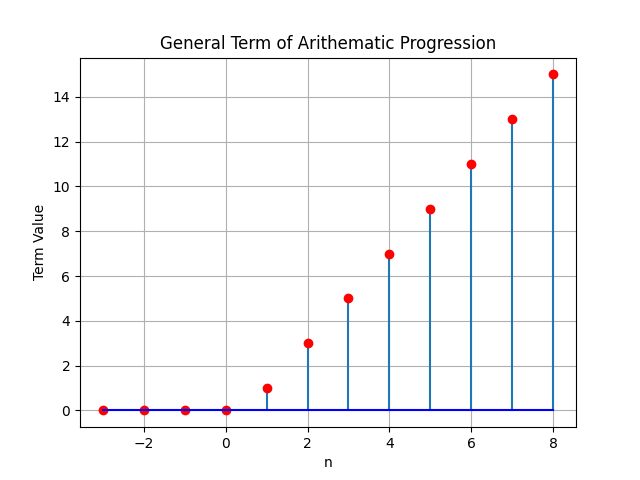
\includegraphics[width=1.0\linewidth]{Figure_2.png}
    \caption{Plot of general term of AP taken from Python}
    \label{fig:1}
\end{figure}
The Z-Transform Equation for x\brak{n} is 
\begin{align}
    X\brak{z}&=\sum_{-\infty}^{\infty}\brak{2n-1}z^{-n}u\brak{n} \\
   \implies X\brak{z}&=\sum_{n=0}^{\infty}\brak{2n-1}z^{-n} \\
   \implies X\brak{z}&=\sum_{n=0}^{\infty}\brak{2n}z^{-n} -\sum_{n=0}^{n=\infty}z^{-n}\\
   \implies X(z)&=2\sum_{n=0}^{\infty}\dfrac{n}{z^{n}}-\sum_{n=0}^{\infty}\dfrac{1}{z^{n}}
\end{align}
let us evaluate both the summations separately.let
\begin{align}
   S_\infty&=\sum_{n=0}^{\infty}\dfrac{n}{z^{n}}\\
   \implies \dfrac{S_\infty}{z}&=\sum_{n=0}^{\infty}\dfrac{n}{z^{n+1}}\\
\end{align}
on subtracting both the equations, we get
\begin{align}
   \implies S_\infty\brak{1-\dfrac{1}{z}}&=\sum_{n=0}^{\infty}\dfrac{1}{z^{n}}\\
   \implies S_\infty\brak{1-\dfrac{1}{z}}&=\dfrac{z}{z-1}\\
   \implies S_\infty&=\dfrac{z^2}{\brak{z-1}^{2}}
\end{align}
Now,
\begin{align}
    S_{\infty}^{|}&=\sum_{n=0}^{\infty}\dfrac{1}{z^{n}}\\
    \implies S_{\infty}^{|}&=\dfrac{z}{z-1}
\end{align}
Now to get the desired result,
\begin{align}
    X\brak{z}&=2S_\infty-S_{\infty}^{|}\\
    X\brak{z}&=\dfrac{z^2+z}{\brak{z-1}^{2}}
\end{align}
\begin{table}[h!]
\begin{center}
\renewcommand\thetable{1}
\begin{tabular}{ |c|c|  } 
  \hline
    Parameter & Value  \\ 
  \hline
  First term of A.P $(a_1)$ & 1  \\ 
  \hline
  Common difference (d) & 2 \\ 
  \hline
  The value of m & 14 \\
  \hline
\end{tabular}
\end{center}
\caption{Variables used}
\end{table}
\end{document}
